\chapter{An Ontology for Knowledge-Based Wireless Sensor Networks}\label{chap:ont}
In this chapter, we explain the ontology we have proposed to formally define the components within K-HAS, the structure of the sensed data, the users involved with the network, as well as the format of the sensed data that is passed through the network.

This ontology is for those wanting to deploy a WSN that uses knowledge to classify the ecological observations recorded, or even to select parts of the ontology that meet their requirements and implement those. Terms have been used to map to widely-used ontologies in the domains of ecological observation, sensors and people. However, our proposed architecture (Chapter \ref{chap:arch}) defines new terms that do not exist in current ontologies, thus we extend the alignment of these existing ontologies to create an ontology that encompasses the ontologies as well as defining new terms to match our architecture.

\section{Background}\label{bg}

K-HAS was developed in order to provide a generic architecture for wireless sensor networks to utilise the local knowledge contained within their environment to process sensed data and, therefore, make more efficient use of the network bandwidth by prioritising sensed data that is deemed to be more valuable. We have defined local knowledge as knowledge of an area that has been gained through experience, or experimentation.

Before we were able to implement K-HAS, we needed a high-level model that defined relationships between each tier of the architecture, as well as the data standard used to transport sensed data from DC nodes to an endpoint. Developing an ontology for K-HAS means that we can do this, as well as provide a computer-readable model for all of the classes and components used by K-HAS.

Making it computer readable has allowed us to reuse classes in the development of software for each tier. For example, we were able to develop a common Darwin Core java library that is used in this ontology and in our GSN middleware to unzip and process received archives.

During the development of the K-HAS ontology, we researched existing ontologies that were commonly used in the domains that K-HAS covered. These included scientific observations and sensor hardware.

Looking into these existing ontologies, we found that there had been many surveys on representing sensors in the semantic web: \cite{Compton2009}, \cite{Janowicz2010}, outlines the existing work. These surveys clearly highlighted that these ontologies had been split into two branches; observation-centric and sensor-centric.

Observation-centric ontologies, such as OBOE \cite{Madin2007b} and O\&M \cite{botts},  focus on the data that is sensed, and its content; whereas sensor-centric ontologies, such as SSN \cite{Compton2012} and SensorML\cite{botts}, detail the components that make up a sensor and the operations they perform to turn sensed data into an output.

% We did find a set of related ontologies that extend the Standard Upper Merged Ontology (SUMO) \cite{niles2001towards}. The three ontologies linked these concepts together to show the flow of data within the network and the role that each sensor plays in delivering this data, discussed later in Section \ref{ont:sumo:sdo}. The reason there are so few could be because other WSNs do not integrate structure, hardware and sensed data in the same way as K-HAS or due to the fact that most WSNs do not process their sensed data until they reach a base station, so they would not need to model their data structure within the network. Because of this, we developed an aligning ontology that reuses existing ontologies, where possible, and introduces new classes that allows these ontologies to interlink. The result is an ontology that covers the flow of sensed data from the point of capture to the point it is received, processed, reviewed and stored at the end point of the network. Not only does the ontology cover how the data changes as it flows through the network but also the roles and capabilities of each tier.

% The Semantic Sensor Ontology, covered in 

K-HAS has been developed to be used with any sensors and is not specific to wildlife cameras, therefore we also looked into sensor-based ontologies that concentrate on the hardware and the individual capabilities of each device within the network.

% From this we have categorised relevant existing ontologies into Observation-Centric and Sensor-Centric ontologies.

\subsection{Observation-Centric Ontologies}

\subsubsection{OBOE}\label{OBOE}
The Extensible Observation Ontology (known in reverse as OBOE) is a popular suite of ontologies used to represent scientific observations \cite{Madin2007b}. Initially starting as base ontology for ecological observations, it has now grown into a suite of extensions that make it suited for chemistry, bioinformatics, anatomy and others. OBOE is represented by OWL-DL \cite{McGuinness2004} and allows the characteristics of a generic scientific observation to be linked to domain specific characteristics.

OBOE focuses on the concept of an \textit{observation}, which is made up of an entity, a measurement and a characteristic \cite{Madin2007}. An example of an observation could be a researcher observing an animal (the entity) and recording the gender (the measurement) as male (the characteristic). A single observation could then consist of multiple observations within it, such as gender, location, species and the number of species observed. 

    \begin{figure}
    \centering
        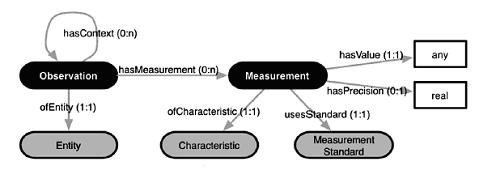
\includegraphics[width=\textwidth]{Chap5/figures/OBOEcore.JPG}
    \caption{The Core of an OBOE Observation \cite{Madin2007}}
    \label{oboe}
    \end{figure}

Figure \ref{oboe} shows the basic structure of a core OBOE observation, outlining the five key classes that are linked by seven properties. While this is the core structure of OBOE, domain specific extensions have been implemented by utilising `extension points' that are part of OBOE's core. OBOE follows the O\&M Standard (below) very closely, providing extensions to the core classes that allows more information about each to be encoded, adding context and enhancing the value of an observation.

The primary benefits of OBOE are that it is generic enough to cover almost all types of scientific observation and domain extensions allow for more specific details to be stored.

\subsubsection{O\&M}
The Open Geospatial Consortium (OGC) Observations and Measurements Standard aims to provide a framework suitable for recording any observation made by a sensor, regardless of the domain \cite{botts}. 

A key feature of O\&M is that \textit{observation} and \textit{measurement} are not just classes. They also denote an action.
An observation is an action that causes a result, yielding a value and a measurement is a set of operations that provide some result(s).

O\&M provides a conceptual model, as well as XML encoding for observations and measurements. The listing \ref{omxml} shows an observation of a vehicle in a given time and place. Similar to the encoding of a measurement with the standard and protocol used in OBOE, O\&M provides support for the recording of the procedure used to gain the measurement for the observation. 
\vspace{\baselineskip}
\begin{lstlisting}[caption=An Observation of a Vehicle encoded in O\&M, label=omxml, breaklines=true, language=XML]
 <?xml version="1.0" encoding="windows-1250"?>
 <om:GeometryObservation gml:id="geom1610" 
 xmlns:om="http://www.opengis.net/om/1.0" 
 xmlns:xsi="http://www.w3.org/2001/XMLSchema-instance" 
 xmlns:xlink="http://www.w3.org/1999/xlink" 
 xmlns:gml="http://www.opengis.net/gml" 
 xsi:schemaLocation="..Specialization_override.xsd">
   <om:samplingTime>
     <gml:TimeInstant>
       <gml:timePosition>2009-09-16T17:22:25.00</gml:timePosition>
     </gml:TimeInstant>
   </om:samplingTime>
   <om:procedure xlink:href="urn:ogc:object:procedure:ifgi:GPS"/>
   <om:observedProperty xlink:href="urn:ogc:def:phenomenon:OGC:Shape"/>
   <om:featureOfInterest xlink:href="urn:ogc:object:feature:vehicle"/>
   <om:result>
     <gml:Point srsName="urn:ogc:crs:epsg:4326">
       <gml:pos>40.7833 -73.9667</gml:pos>
     </gml:Point>
   </om:result>
 </om:GeometryObservation>
 \end{lstlisting}
 
 The listing shows that an observation centres around a \textit{feature of interest} that can be a physical object and the measurement is the detection of the vehicle at the recorded location. Figure \ref{oandm} shows a basic diagram of the ontology. While the event of a feature is linked, it is clear that the main focus is on the observation and the measurement associated with it.

    \begin{figure}[h]
    \centering
	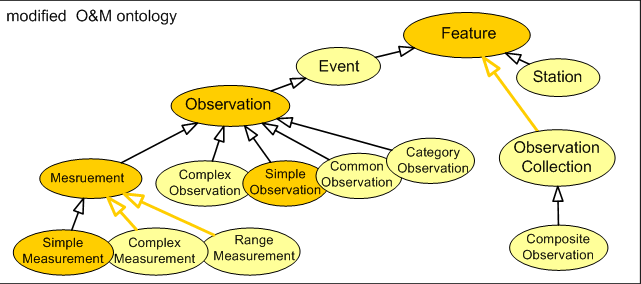
\includegraphics[width=\textwidth]{Chap5/figures/o&m_ontology.png}
    \caption{The OGC O\&M Ontology \cite{Probst}}
    \label{oandm}
    \end{figure}
 
The structure of an observation within O\&M is focussed on the action and the result, this makes it suited for sensor networks across many domains that perform a wide range of observations. Because the users of the O\&M standard are spread across many domains, each with their own terms and definitions, the creation of an ontology for the standard aimed to remain as generic as other observation-centric ontologies. 

\subsubsection{Darwin Core SW}\label{bg:dwc}

In order to represent DwC occurrences, covered in Section \ref{arch:tech:dwc}, in an ontological format, work has been done to represent Darwin Core terms, as an ontology, in OWL. Darwin-Semantic Web (Darwin-SW) \cite{Baskauf} is the project that aims to do this and many of the core terms associated with an occurrence have already been formalised and Figure \ref{darwin-sw} shows the entity relationship model of these terms.

    \begin{figure}[h!]
    \centering
  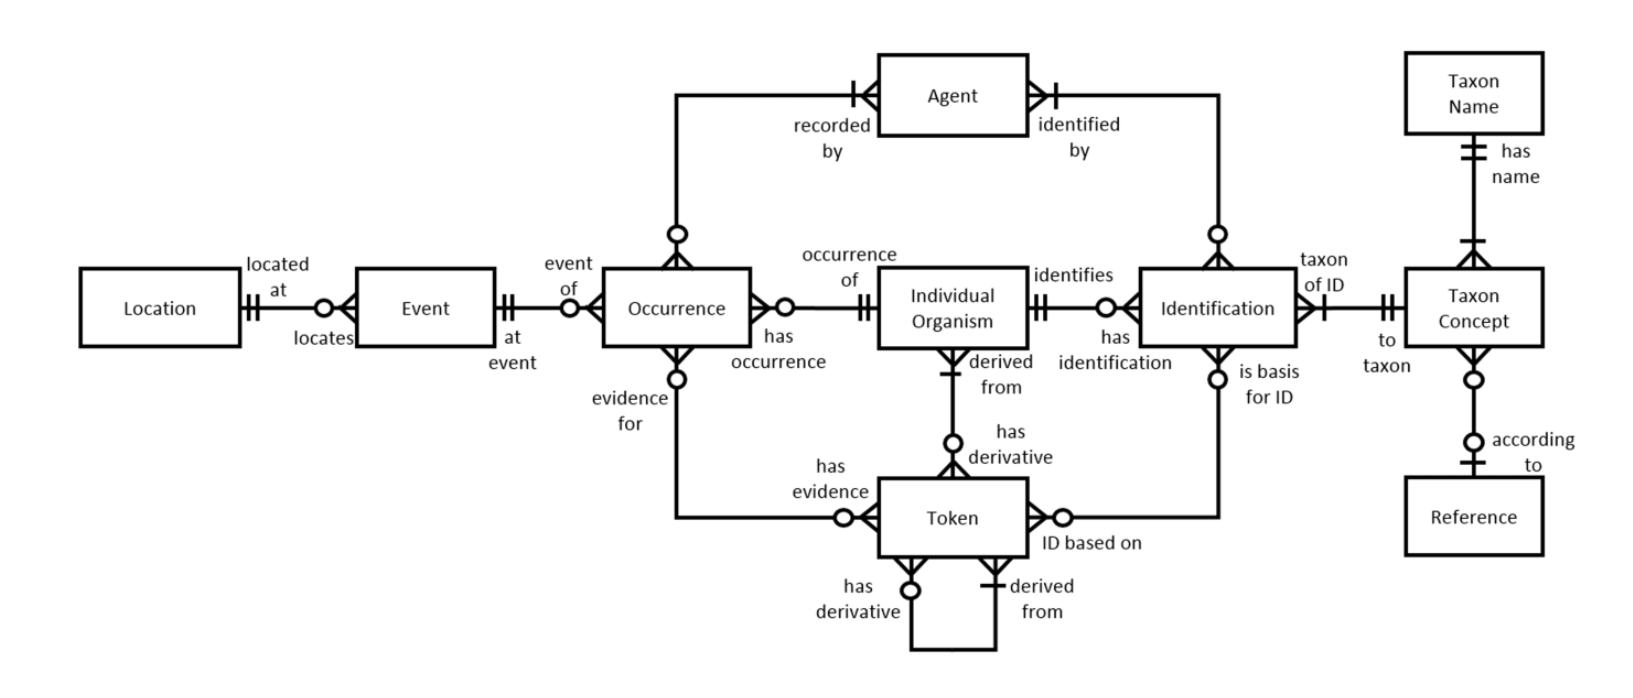
\includegraphics[width=\textwidth]{Chap5/figures/darwinsw}
    \caption{Darwin-SW Entity-Relationship Model \cite{Baskauf}}
    \label{darwin-sw}
    \end{figure}

While Darwin-SW does not represent all of the classes within the DwC namespace, it contains the core classes required to record an occurrence, to a more-detailed level than OBOE. The downside of this is that the specificity of the terms limits DwC to ecological observations, making it far less generic than OBOE and other alternatives. There are positive aspects that, for those that need to record ecological observations, DwC allows for a greater level of detail and  can be mapped to OBOE with ease.

Listing \ref{ont:darwinsw} shows a fragment of a DwC occurrence of a living specimen which, in this case, is a tree \cite{Baskauf2011}. Darwin-SW, and Darwin Core, terms are used to describe the identification of the tree, such as the by whom it was identified, the date and the taxon. The full source can be seen in Appendix \ref{appendix:dsw} and includes links to existing related occurrences, other images of the individual and relationships to other resources.
\vspace{\baselineskip}
\begin{lstlisting}[caption={Darwin-SW Representation of an Identification}, label={ont:darwinsw}, language=XML]
<dsw:hasIdentification>
  <rdf:Description rdf:about="http://bioimages.vanderbilt.edu/vanderbilt/12-126#2002-04-10baskauf">
        <dcterms:description>Determination of Ginkgo biloba L. sensu Flora of North America (1993) for the individual http://bioimages.vanderbilt.edu/vanderbilt/12-126</dcterms:description>
        <rdf:type rdf:resource="http://rs.tdwg.org/dwc/terms/Identification" />
        
        <!-- In lieu of stable external identifiers for taxon concepts, Im defining some onsite -->
        <dsw:toTaxon rdf:resource="http://bioimages.vanderbilt.edu/taxonConcepts#183269-fna1993" />
        
        <dwc:identifiedBy>Steven J. Baskauf</dwc:identifiedBy>
        <dsw:idBy rdf:resource="http://bioimages.vanderbilt.edu/contact/baskauf" />
        <dwc:dateIdentified>2002-04-10</dwc:dateIdentified>
        
        <!-- Relationship of the identification to other resources -->
        <dsw:idBasedOn rdf:resource="http://bioimages.vanderbilt.edu/baskauf/10554"/>
  </rdf:Description>
</dsw:hasIdentification>
\end{lstlisting}

\subsection{Sensor-Centric Ontologies}
Sensor-centric ontologies are more focussed on the structure of the sensor, the network and the sensing processes involved. 

\subsubsection{SensorML}
The Sensor Markup Language (SensorML) Standard has been developed by the OGC, and complements the O\&M Standard, to enable the discovery and tasking of internet-connected sensors \cite{botts}.

SensorML provides an XML schema for describing a sensor, its capabilities and the processes available. At the core, SensorML comprises of:
\begin{enumerate}
  \item Component - A physical process that transforms information from one form to another.
  \item System - Model of a group of components.
  \item Process Model - Atomic processing block used within a Process Chain.
  \item Process Chain - Composite block of Process Models.
  \item Process Method - Definition of the behaviour of a Process Model.
  \item Detector - Atomic part of a Measurement System.
  \item System - Array of components, relates a Process Chain to the real world.
  \item Measurement System - Specific type of System, mainly consisting of sampling devices and detectors.
  \item Sensor - Specific type of System that represents a complete Sensor.
\end{enumerate}

These definitions outline the core concepts of SensorML, a \textit{system} that performs one (or more) process(es) and is comprised of a group of \textit{components} \cite{Robin2006}. A SensorML document allow for a general, formal specification of a \textit{sensor} and its capabilities. The document describes a \textit{component}, outlining what data it reads in and the output once it has been processed. Several of these \textit{components} can the be used to create a \textit{system} and the primary goal of SensorML is to describe the process of how an observation came to be, focussing on the technical features of the node.

%\begin{lstlisting}[caption=SensorML Sample Document, label=sensormldoc, breaklines=true]
%<Component>
%  <keywords>
%    <KeywordList>
%      <keyword>weather station</keyword>
%  ...
%    </KeywordList>
%  </keywords>
%  <identification>
%    <IdentifierList>
%      <identifier name="uniqueID">
%        <Term definition="urn:ogc:def:identifier:OGC:uniqueID">
%          <value>urn:ogc:object:feature:Sensor:IFGI:thermometer123</value>
%        </Term>
%      </identifier>
%  ...
%      </identifier>
%    </IdentifierList>
%  </identification>
%  <classification>
%    <ClassifierList>
%      <classifier name="sensorType">
%        <Term definition="urn:ogc:def:classifier:OGC:1.0:sensorType">
%          <value>thermometer</value>
%        </Term>
%      </classifier>
%    </ClassifierList>
%  </classification>
%  <capabilities>
%    <swe:DataRecord definition="urn:ogc:def:property:capabilities">
%      <swe:field name="status">
%        <swe:Text definition="urn:ogc:def:property:OGC:1.0:status">
%          <gml:description>System operating values.</gml:description>
%          <swe:value>active</swe:value>
%        </swe:Text>
%      </swe:field>
%    </swe:DataRecord> 
%  </capabilities>
%  <inputs>
%    <InputList>
%      <input name="atmosphericTemperature">
%        <swe:ObservableProperty definition="urn:temperature"/>
%      </input>
%    </InputList>
%  </inputs>
%  <outputs>
%    <OutputList>
%      <output name="temperature">
%        <swe:Quantity definition="urn:ogc:def:property:OGC:1.0:temperature">
%          <gml:groupName codeSpace="ObservationOffering"> Weather </gml:groupName>
%          <swe:uom code="Cel"/>
%        </swe:Quantity>
%      </output>
%    </OutputList>
%  </outputs>
%</Component>
%  \end{lstlisting}

\subsection{Combined Sensor and Observation Ontologies}
In this section, we review ontologies that represent the hardware of the sensors within a network, as well as the observations they record. This allows them to model the sensing capabilities of each sensor, the measurements they capture and the data they record.

\subsubsection{SSN}
The Semantic Sensor Network (SSN) Ontology is the most fitting ontology for our requirements, as it covers systems processes and observations. Developed by the W3C after an extensive review of existing ontologies \cite{Compton2012}, the SSN ontology is designed to allow focus on a variety of perspectives, such as the sensor within the network or the data that has been observed.

    \begin{figure}[h]
    \centering
        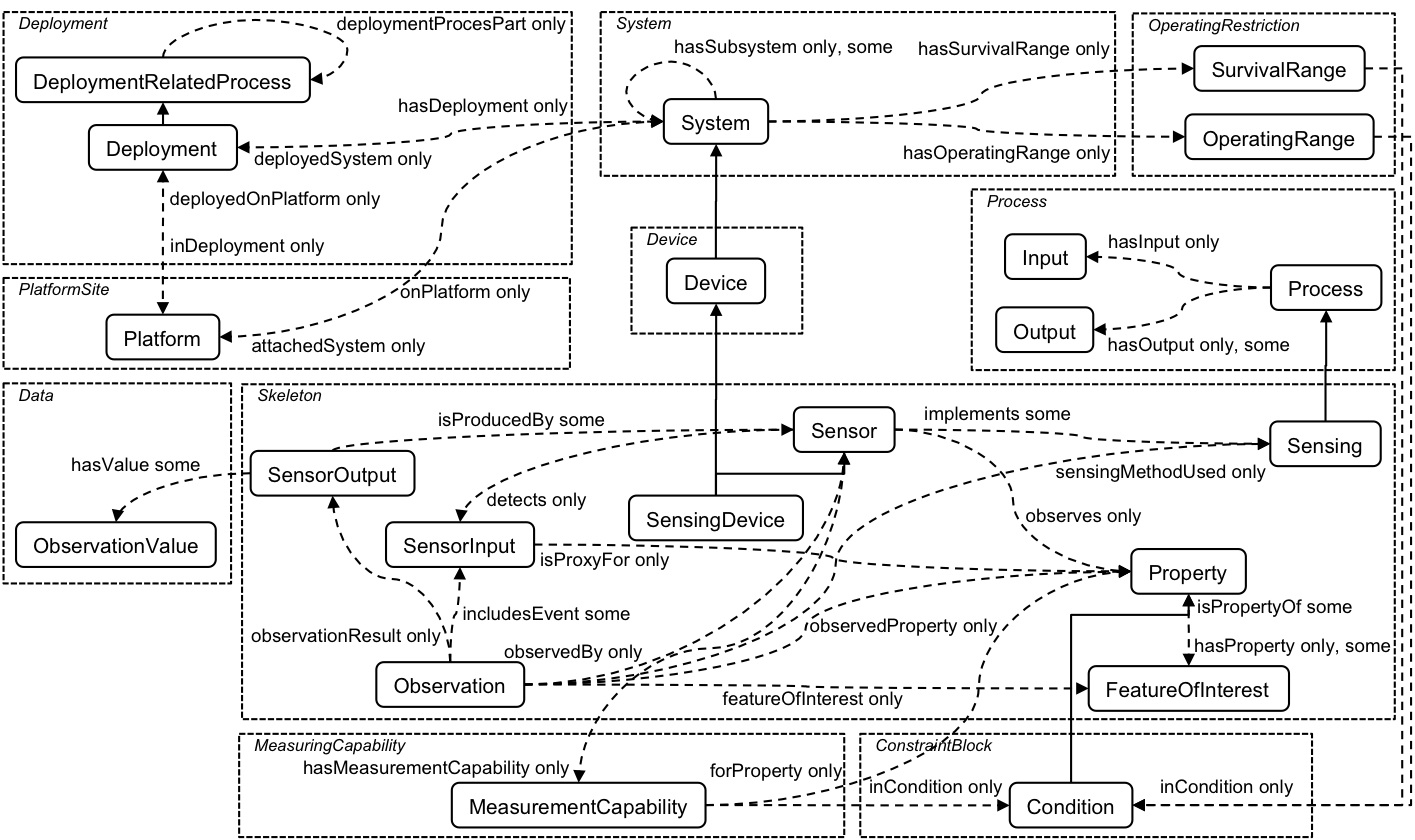
\includegraphics[width=\textwidth]{Chap5/figures/ssnont.jpg}
    \caption{SSN Ontology}
    \label{ssnont}
    \end{figure}
    
Figure \ref{ssnont} shows the model for the SSN ontology, displaying the relationships that connect each class, as well as their associated properties. It also highlights the modular approach that has been taken, separating the system from the process and the observation.

The observation pattern of SSN is centred around `Stimuli-Sensor-Observation', which can be simply described by an event causing a sensor to trigger and create an encompassing observation to store details about the event, as well as the device that recorded the event. While SSN is focussed on sensors, capturing the measurement capabilities of each sensing device that makes up a system and specifics on its lifespan, the development of the ontology arose from the review of sensor-centric ontologies as well, recording data about observations in a structure very similar to O\&M.

\subsubsection{SUMO Extension}\label{ont:sumo:sho}
The Suggested Upper Merged Ontology (SUMO) is a general purpose ontology \cite{niles2001towards} that provides general-purpose terms and is intended to be extended for domain specific ontologies. In \cite{Eid2007}, SUMO has been extended to link sensor hardware and sensor data ontologies in order to assist with searching and evaluating distributed and heterogenous sensor networks. The work combines the Sensor Hierarchy Ontology (SHO), the Sensor Data Ontology (SDO) and the ability to `plug in' extension ontologies.

The SHO describes the hardware of a sensor node, as well as its accuracy, transmission medium and data processing capabilities. The SDO, however, describes the sensing properties of a device beyond the hardware and the context of the sensor can be enriched with information about spatial and/or temporal observations. Similar to GSN (Section \ref{sec:GSN}), SUMO uses the notion of virtual sensors where a group of sensors can be described together to provide abstract measurements. In \cite{Eid2007}, the example of a humidity sensor, temperature sensor and wind speed sensor being collectively described as \textit{weather sensors}.
The SHO ontology is another extension of SUMO, from \cite{Eid2007}, that represents the hardware of a WSN, including the node itself, data transmission units, data processing units and individual sensors. The data model describes a sensor with metadata describing features such as measurement type, transmission range and physical properties.


\subsection{Findings}
There are many ontologies that are suited for sensor-based scientific observations and ontologies that allow for the description of sensor hardware cover the hardware capabilities of sensors as a whole and sensor systems comprised of multiple sensors in great detail. SSN and SUMO were the closest that we found for this, but SSN was still very hardware focused and went into greater detail of the hardware capabilities of each measuring devices than we needed. 
%SSN's focus on the hardware of each node and their capabilities is different to our requirements for both hardware and sensed data to be represented in a single ontology. 

While the SHO and SDO extensions of SUMO are classed as both an observation-centric and sensor-centric ontologies, they are separate ontologies that model both sensor hardware and sensed data and, while the development of these ontologies did follow a similar approach to the one described in this chapter (combining ontologies), the core concepts of SHO and SDO are more focussed on retrieval of sensed data through queries constructed using both hardware details and properties of the sensed data.
 %does not fulfil all of the requirements we identified when developing K-HAS, such as representing users. 
However, an important feature is the Extension Plugin Ontologies (EPO), support for domain specific plugins to integrate with SUMO and integrate with the SHO and SDO and this would also be a useful feature for K-HAS.

\section{Method}
We found that SSN, SensorML and Darwin Core satisfied many the hardware and much of the sensed data subsections of K-HAS completely. We have used these existing ontologies to develop an aligning ontology that connects ontologies across multiple domains to support our proposal of K-HAS, extending the concepts in existing ontologies with K-HAS specific concepts.

%SSN DISCUSSION HERE!
The SSN ontology is a modular ontology created by combining concepts from existing, commonly used ontologies and allows for domain specific concepts to be imported. Some of the main uses cases for the SSN ontology are provenance and data discovery, which are also key within K-HAS. However, the tiered structure of K-HAS did not map directly to SSN and it proved difficult to represent the flow of knowledge through a network, as humans can also perform similar operations on observations and the observations are enriched as they pass through the network. However, while we did not use the ontology directly, many of the concepts can be mapped directly (shown later in Table \ref{tab:dwc_eval}) and it would be possible to use import modules from SSN and extend them with the concepts specific to K-HAS, SSN does not describe domain concepts (such as time or location) as this is expected to be handled by imports from more specific ontologies. K-HAS allows humans to act as sensors, which would require slight modifications to SSN, as well as extending with the ability to provide classifications for sensed data.

%Mappings table here!


 %The majority of the concepts described can be mapped to K-HAS and the observation-centric terms could be further extended to incorporate Darwin Core observations. However, when developing the K-HAS ontology, our focus was on the flow of knowledge through the network and we found that the SSN ontology definded sensing nodes as devices capable of sensing their environment and some processing capabilities, but not as devices that enriched the data they sensed with further knowledge. Many of the terms used in K-HAS map directly to SSN and one of the goals of SSN to show provenance is something we would like to implement in the K-HAS ontology. 

% *Outline standard ontology development method
% *Explain our variation
% Reference the various methods outlined

Before we began development, we researched existing methods that have been used to develop current ontologies. From this, we found three well-documented methodologies; the methodology used to develop the Toronto Virtual Enterprise (TOVE) ontolgy, the Methontology and the methodology used to develop the Enterprise Model ontology.

The methodology by Uschold and King \cite{Uschold1995}, used to develop the Enterprise ontology, is a four step method that was most suited to the processes we expected to follow. The steps are not covered in great detail in the original paper but, research since provides greater detail for each step.

\subsection{Identify Purpose}
The aim of this step is to identify why the ontology is being built and what requirements it is supposed to fulfil. This includes considerations, such as the audience, the intended purpose and the specificity of the ontology.

Other methodologies have used more structured methods to informally identify the requirements of the ontology. Gruninger and Fox \cite{Gruninger1995} propose competency questions; these are questions that are used to identify the problems that the developed ontology is developed to solve. These questions can act as a benchmark, showing that an ontology is sufficient if it can solve the questions raised here.

\subsection{Build the Ontology}
Building the ontology can be broken down further into 3 smaller steps: capture, code and integrate existing ontologies.

\subsubsection{Capture}
 % - identify key concepts, provide unambiguous text definitions
The capture stage involves defining the concepts and terms that the ontology will model, as well as how they map to the real world. This can be done in one of three ways:
\begin{enumerate}
\item Top Down - Starting with the core concepts, create the more specialised classes until you have identified all subclasses.
\item Bottom Up - This process begins with the more specialised classes and grouping them into the more general classes towards the top of the hierarchy.
\item Middle Out - A combination of the two, this process involves specialising, and generalising, the classes identified in the middle layer of the hierarchy.
\end{enumerate}
% REFERENCE THE ONTOLOGY 101 PAPER
As for the capture of the knowledge used to identify the classes needed, this is an area that has been documented, but primarily provides recommendations. \cite{Fernandez-Lopez1999} suggests interviews with domain experts, iteratively brainstorming with a group actively involved in the development of the ontology. This stage has often been referred to as the knowledge-acquisition stage.
% and **REFERENCE** recommends the use of Common KADS \cite{Hoog1992}, a knowledge analysis methodology used to develop knowledge-intensive systems.

\subsubsection{Code}
 % - perform the above step in a formal language (i.e. OWL)
This step involves coding the terms identified in the previous step into a formal language, such as the Web Ontology Language (OWL) \cite{McGuinness2004}.

\subsubsection{Integrate Existing Ontologies}
 % - join all ontologies that match/overlap with the identified terms
This step can be carried out at the same time as the step above, so that the ontology is developed with existing ontologies in mind. This also allows overlap to be identified, and incorporated, early. Being aware of commonly-used ontologies within the domain, before development begins, is a more logical approach and does avoid the need to create new terms for existing concepts.

Existing ontologies can be integrated by importing them and linking the existing terms to the terms identified in the ontology that is being developed. However, there is also the method of developing the ontology completely, so that it is consistent without the need to rely on existing ontologies and creating `sameAs' relationships between the terms identified and only the required terms in the existing ontologies.

In \cite{Jimenez-Ruiz2008}, it is recommended that, when importing external ontologies, the whole ontology is not used. Rather, one should aim to extract only the required fragments from the external ontology that are relevant to the concepts in the developed ontology.


\subsection{Evaluation}\label{method:eval}
For the evaluation, Uschold and King adopt the definition of \cite{Fernandez-Lopez1997}: `to make a technical judgement of the ontologies, their associated software environment, and documentation with respect to a frame of reference... The frame of reference may be requirements specifications, competency questions, and/or the real world'.

There are some well documented methods for evaluating ontologies in the literature, \cite{Uschold} proposes using the competency questions, used in the first step, to ensure that they can all be fully answered by the finished ontology. 

\subsection{Documentation}
Although this step is listed at the end of the development cycle, it seems more fitting to document all major aspects of the ontology as it is being developed. Documentation of the ontology should include: any assumptions, all concepts introduced, all ontologies that have been incorporated (by whatever means) and any primitives used for the definitions of concepts.

\section{Results}
This section details our results when using the Uschold and King methodology, accompanied by more recent research for particular steps, to develop the K-HAS ontology. 

\subsection{Identify Purpose}\label{ident}
The need to create the K-HAS ontology was partly due to the reasons outlined by Gruninger and Fox \cite{Gruninger1995}, we had identified a problem as we were developing a sensing architecture that utilised local knowledge: how could we formally represent the flow of knowledge and sensed data throughout a wireless sensor network?

To determine the scope that K-HAS should cover, we identified a set of competency questions that represent what we expect K-HAS to cover within the domain. In order to present this, we used an approach similar to that of \cite{Choi2010}, which can be seen in Table \ref{tab:comp_qs}.

\begin{table}[ht!]
\centering
\begin{tabular}{ p{10cm}}
\hline
\textbf{Competency Questions}\\ 
\hline
Find all \textbf{Occurrences} of an \textbf{Individual} \\
Find all \textbf{Occurrences} of an \textbf{Individual} at a \textbf{Location}\\
Find all \textbf{Occurrences} within a specified \textbf{Date} and \textbf{Time} range \\
Find all \textbf{Sensors} that have recorded an \textbf{Occurrence} of an \textbf{Individual}\\ 
Find all \textbf{Locations} of an \textbf{Individual}  \\
Find the storage location of a \textbf{Project} \\ 
Find all \textbf{Projects} containing an \textbf{Individual}\\
Find all \textbf{People} involved in a \textbf{Project}  \\
Find all the \textbf{Evidence} that supports an \textbf{Occurrence}\\
Find all the \textbf{Types} of evidence that supports an \textbf{Occurrence} \\
\hline 
\end{tabular}
\caption{Competency Questions} 
\label{tab:comp_qs}
\end{table} 

These questions allow us to identify the core concepts that the ontology needs to represent, as well as serving as a tool to evaluate the completed ontology.

\subsection{Build the Ontology - Capture}\label{buildcapture}
This part of the development cycle is the identification of the concepts and their implementation. The first step is capture the knowledge that will be used to identify the core concepts within the ontology. 

To capture the knowledge for the ontology, we used a combinatorial approach of those outlined in the literature. We interviewed domain experts, as well as overseeing a basic implementation of a system, and we iteratively brainstormed the concepts throughout the development cycle.

Over the course of eighteen months, which involved 2 field visits and several brainstorming meetings, we identified the core concepts that the ontology would need to contain, as well as the properties that would link them. From this, it would seem that we followed the \textit{Top-Down} approach, but the first visit with domain experts also allowed us to identify some of the more specialist classes early on in the development cycle. Thus, it seems that in practice we followed a more \textit{Middle-Out} approach.

Table \ref{tab:concepts} outlines the core concepts we have identified for K-HAS to be complete, as well as the definitions we have used for the architecture. When integrating existing ontologies, the definitions of similar terms would need to match with our definitions or we would not deem them the same as the K-HAS concepts.

\begin{table}[ht!]
\centering
\begin{tabular}{|p{5cm}|p{2cm}|p{5cm}|}
\hline
\textbf{Concept} & \textbf{Subclass Of} & \textbf{Definition}\\ 
\hline
Occurrence & - &  \\
Identification & - &  A text-based recording of the content of an Occurrence\\
Evidence & - & Media to support the Identification, such as a photo or recording.\\
Location & - & The location of the Occurrence.\\ 
Date & - & The date of the Occurrence.\\
Time & - & The time of the Occurrence.\\ 
Project & - & Project(s) that can contain many Occurrences\\ 
Node & - & A device with sensing capabilities.\\ 
Data Collection (DC) Node & Node & Node with limited knowledge-processing capabilities charged with sensing a feature (or features) of its environment. \\
Data Processing (DP) Node & Node & Node with knowledge-processing capabilities charged with serving a subset of DC Nodes and processing their sensed data. \\
Data Aggregation (DA) Node & Node & Node with knowledge-processing capabilities that stores all knowledge and sensed data for the whole network. \\
Person & - &\\ 
Administrator & Person & Person in charge of a project (or projects). \\
Worker & Person & Person involved with a project. \\
\hline 
\end{tabular}
\caption{K-HAS Concepts} 
\label{tab:concepts}
\end{table}

Mapping these concepts, a diagram of the base K-HAS ontology is shown in Figure \ref{khas_base_ont}. The next step is to create the ontology and map the concepts identified to existing ontologies within the same domain space(s).

    \begin{figure}[H]
    \centering
        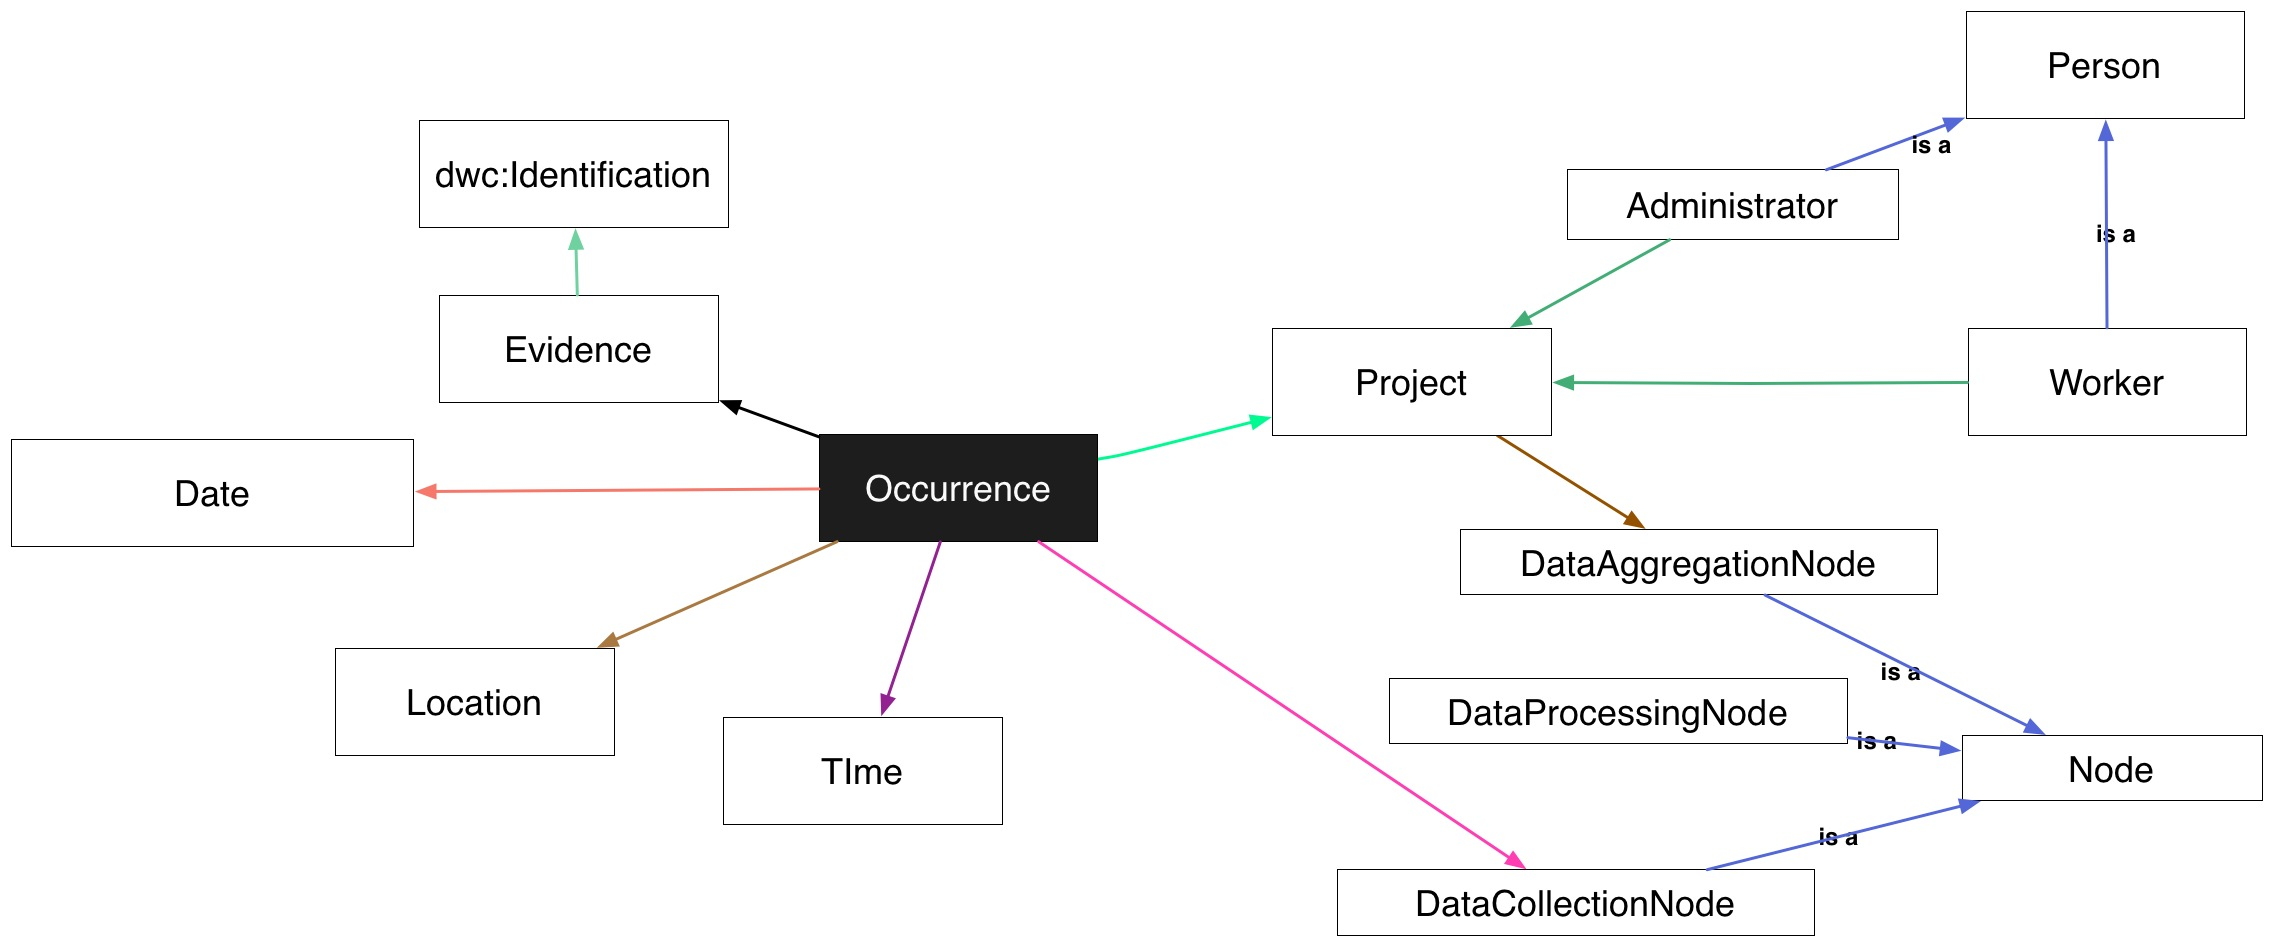
\includegraphics[width=\textwidth]{Chap5/figures/khas_base.JPG}
    \caption{K-HAS Base Ontology}
    \label{khas_base_ont}
    \end{figure}



\subsection{Build the Ontology - Code}
Once the concepts had been identified (and agreed upon), the ontology must be coded. We used Protege 4.2.2 \cite{Noy2000a} and implemented K-HAS in the Web Ontology Language (OWL), creating a core file that could be expanded; should we need to import existing ontologies.

\subsection{Build the Ontology - Integrate Existing Ontologies}
Our proposal for K-HAS is focused on scientific observations. Because of this, the focal point of our existing ontology research is on ontologies that are centred around scientific observations. This allows us to create a more generic ontology that is still able to capture all of the semantic details associated with a wildlife observation.

As explained in Section \ref{bg}, our research of existing ontologies covered two categories: observation-centric and sensor-centric. We identified ontologies, within multiple domains, that satisfied many of our requirements for K-HAS, but not all. Using the core concepts outlined in Section \ref{buildcapture}, we created a minimal ontology and used the results of our research to map K-HAS concepts to those that had already been identified.

During this process we found that we had determined concepts that mapped to existing ontologies, but may not share identical structures, or even the same name. For example, the OBOE ontology describes the concept of an occurrence, which is very similar to our occurrence and the occurrence in the Darwin Core-SW ontology. When we found these mappings, we used \textit{sameAs} relationship to form a link that allows data stored according to these existing ontologies to map directly to K-HAS. However, the structure of an OBOE observation is, as outlined in Section \ref{OBOE}, more generic for all types of scientific observation and depicts the observation of an entity, containing a measurement of a particular characteristic. Whereas the structure of a Darwin Core observation is more limited to scientific observations of taxa which allows it to have more predefined terms, such as location, species name and the evidence for the recorded individual. Because of this, it was difficult to create a structure that encapsulated both OBOE and Darwin Core due to the generality of an OBOE observation compared to the more specific structure of DwC.

Research showed that Darwin Core maps to K-HAS' requirements more completely, as well as the fact that there has been work to represent Darwin Core Observations in OBOE \cite{dwc_oboe}, K-HAS occurrences map directly to Darwin Core and elements that are similar to OBOE have been linked by the \textit{sameAs} relationship. This does mean that full OBOE observations cannot map directly, but K-HAS, and Darwin Core, occurrences can be converted, if necessary. However, using the terms in our ontology we can create a subset of an observation that does not include all of the terms defined in OBOE but can still map to all three ontologies.

For the sensor hardware of K-HAS, we found that the SensorML ontology maps directly to our concepts and we also realised that we did not need to recreate concepts that may already exist in popular ontologies outside of the domain spaces we researched. For example, the Friend of a Friend (FOAF) ontology \cite{Document2010} is an ontology designed to create machine-readable pages that describe people, so it is more logical that K-HAS reuses existing terms from popular ontologies to allow pre-existing data to be mapped with ease.

% INCLUDE TABLE TO MATCH TERMS TO EXISTING ONTOLOGIES??

\subsection{Extend the Ontology}

Whilst researching widely-used ontologies, we became aware that some classes identified for K-HAS were not satisfied by what is currently available, these are prefixed with khas and shown in Figure \ref{khas_ont}. The final step for creating the ontology was to add these concepts to the linked ontologies, we call these \textit{extension concepts}, concepts unique to K-HAS which do not exist in any other ontology. These terms were linked to the unique layered architecture of K-HAS and we defined them within a new K-HAS namespace, changing our ontology from an alignment of existing ontologies to an extension of these.

The final ontology is shown in Figure \ref{khas_ont} (with the complete code in Appendix \ref{appendix:ontology}) and shows how each concept maps to existing ontologies. The figure shows that there were only five extension concepts unique to K-HAS that can be subclassed from the \textit{person} concept in the FOAF ontology and \textit{node} in the SensorML ontology.

    \begin{figure}[H]
    \centering
        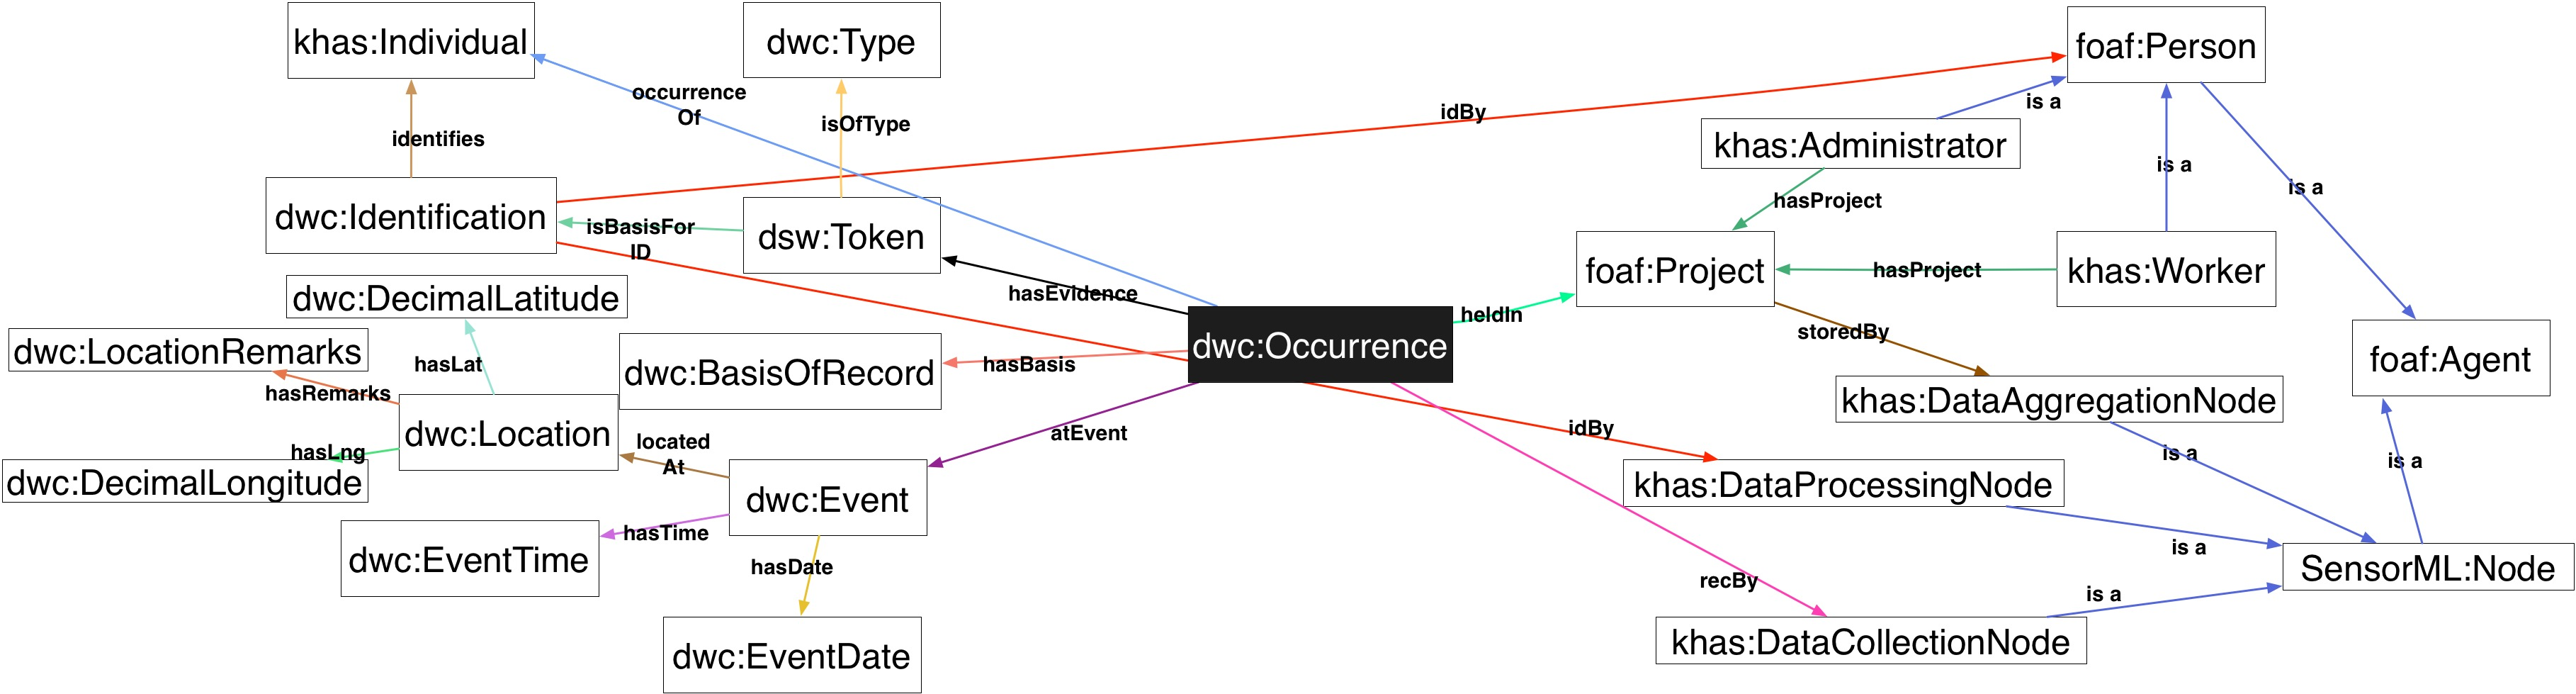
\includegraphics[angle=90, width=\textwidth, height=\textheight, keepaspectratio]{Chap5/figures/khas_ontology_copy.jpg}
    \caption{K-HAS Ontology}
    \label{khas_ont}
    \end{figure}
    
\section{Evaluation}

Uschold and King's ontology development method does not explain how to evaluate the created ontology and much of the literature describes a number of methods that can be employed, \cite{Brank2005} outlines a number of different evaluation techniques and separates them into categories. These categories are listed below:
\begin{enumerate}
	\item Comparing the ontology to a `golden standard'.
	\item Using the ontology in an application and evaluating the results.
	\item Comparing the ontology with a collection of documents from the domain to be covered.
	\item Manual evaluation by humans to test if the ontology meets a set of predefined criteria.
\end{enumerate}

The last category mentioned is similar to the method in Section \ref{method:eval} that uses the competency questions to determine the effectiveness of the ontology. Because there is no agreed method,we have evaluated K-HAS by testing it in the application it was developed in (Protege), mapping it to existing documents within the intended domain and ensuring that it can satisfy all of the competency questions we outlined in Table \ref{tab:comp_qs}.

\subsection{Using the Ontology in an Application}
We developed the K-HAS ontology in Protege, a Java based ontology editor, that also provides the functionality to reason over the ontology and check for inconsistencies. Using the Hermit reasoner that is built into Protege, the ontology was determined to be logically consistent.

To confirm the validation provided by Protege, we also used a web-based ontology validation tool, called the OntOlogy Pitfall Scanner (OOPS), that scans an ontology for common errors, such as defining incorrect inverse relationships or using recursive definitions, that can occur during the development phase \cite{Poveda-Villalon2012}. The results of this tool showed that no pitfalls had been detected.

We have a customised build of K-HAS running that receives data from a variety of sources and stores it in a MySQL database that allows users to classify through a web site. The schema of the database maps to our ontology, scientific observations are received, unzipped and stored in the relevant fields in the database. Using real sensed data, we have successfully stored over two hundred occurrences and mapped existing DwC occurrence to K-HAS.

\subsection{Competency Questions}

In Table \ref{tab:comp_qs} we have identified some basic competency questions that we expected K-HAS to be able to satisfy with the concepts we had identified, Table \ref{eval:comp_qs} shows how the original questions are satisfied by K-HAS. We have mapped the terms we originally used to the terms used in K-HAS (and the linked ontologies) and shown the concepts involved with each question, as well as the relationships linking them.
\begin{table}[H]
%\centering
\begin{tabular}{|p{5cm}|p{4cm}|p{4cm}|}
\hline
\textbf{Competency Questions} & \textbf{Concepts} & \textbf{Relationships}\\ 
\hline
Find all \textbf{Occurrences} of an \textbf{Individual} & Occurrence; Individual & Occurrence occurrenceOf Individual \\
Find all \textbf{Occurrences} of an \textbf{Individual} at a \textbf{Location} & Occurrence, Token, Individual, Location, Identification & Occurrence hasEvidence Token \\ 
& & Token isBasisForID Identification \\ 
& & Identification identifies Individual \\
Find all \textbf{Occurrence} within a specified \textbf{Date} and \textbf{Time} range & Occurrence; Event; Date; Time & Occurrence atEvent Event \\
& & Event hasTime Time \\ 
& & Event hasDate Date \\
Find all \textbf{Data-Collection Nodes} that have recorded an \textbf{Occurrence} of an \textbf{Individual} & DCNode; Individual; Occurrence & Occurrence recordedBy DCNode \\
& & Occurrence occurrenceOf Individual \\  
Find all \textbf{Locations} of an \textbf{Individual} & Occurrence; Individual; Event; Location & Occurrence occurrenceOf Individual \\ 
& & Occurrence hasEvent Event \\ 
& & Event locatedAt Location \\
Find the storage location of a \textbf{Project} & Project, Data Aggregation Node & Project storedBy DataAggregationNode \\ 
Find all \textbf{Projects} containing an \textbf{Individual} & Individual, Project; Occurrence & Individual occurredIn Occurrence \\ 
& & Occurrence heldIn Project \\
Find all \textbf{Persons} involved in a \textbf{Project} & Person; Administrator; Worker; Project & Administrator hasProject Project \\ 
& & Worker hasProject Project \\
Find all the \textbf{Evidence} that supports an \textbf{Occurrence} & Occurrence; Token & Occurrence hasEvidence Evidence \\
Find all the \textbf{Types} of evidence that supports an \textbf{Occurrence} & Occurrence; Token; Type & Occurrence hasEvidence Token \\ 
& & Token isOfType Type \\
\hline 
\end{tabular}
\caption{Competency Questions} 
\label{eval:comp_qs}
\end{table} 

The table shows that all of the competency questions outlined in Section \ref{ident} have been satisfied by the final ontology and each concept used maps quite easily with little to no change.

\subsection{Comparing the Ontology with a Collection of Documents}
Within the domain of scientific observations, Darwin Core is a popular choice for observations of wildlife and plants, it was because of this that we chose to use many of the pre-existing concepts from Darwin Core in K-HAS. 

In the data driven approach suggested by \cite{Brewster2004}, a corpus of documents, related to the domain that the ontology covers, and the keyword content is matched with the terms used in the ontology. Because Darwin Core observations are structured into archives of files, explained in Section \ref{bg:dwc}, we evaluated the K-HAS ontology by combining the approach of comparing a corpus of documents related to the domain with human evaluation of ensuring an ontology met a set of requirements to create a method that ensured existing scientific sensed observations could be mapped to K-HAS with little to no modification.

As explained in Section \ref{arch:tech:dwc}, an archive of Darwin Core files consists of a minimum of 3 files: a metadata file that contains information about the creator of the archive and the project it relates to (eml.xml), a metadata file that describes all of the files that contain the occurrence and the fields within them (meta.xml) and a csv file that contains the data relating to the occurrence itself. Within the archive, the core files that need to be mapped to K-HAS are the meta.xml and eml.xml files as this allows us to store what and who.

We used files from a DwC archive made available online to extract the terms associated with an occurrence and we mapped these terms to K-HAS concepts, the results can be seen in Table \ref{tab:dwc_eval}. This table also shows how K-HAS terms could also be mapped to the SSN ontology.

\begin{table}[H]
\centering
\begin{tabular}{|p{5cm}|p{5cm}|p{5cm}|}
\hline
\textbf{Darwin Core Term} & \textbf{K-HAS Concept} & \textbf{SSN Term} \\
\hline
occurrenceID & Occurrence  & Observation\\
basisOfRecord & Basis of Record & - \\
recordedBy & Person/Node & Observed By \\
associatedMedia & Token & Observation Value \\
eventDate & Event Date & - \\
eventTime & Event Time & - \\
locationId & Location & Region \\
scientificName & Individual & Feature of Interest \\
identifiedBy & Person & -\\
dateIdentified & Identification & - \\
\hline 
\end{tabular}
\caption{Evaluation of K-HAS against Darwin Core Occurrence Terms} 
\label{tab:dwc_eval}
\end{table} 

Each term within a Darwin Core observation maps to K-HAS with only a few changes to the terms, while the definitions do not change. As K-HAS is an alignment ontology, there are extra concepts that do not map to Darwin Core, but can encapsulate each occurrence. For example, a project in K-HAS can contain many occurrences. As previously mentioned, \cite{dwc_oboe} shows how a DwC archive can be represented in OBOE, which means that it would not be too complex to map an OBOE observation in K-HAS.

\section{Conclusion}

In this chapter we have presented an ontology for the K-HAS architecture and described our methodology for development, as well as showing that existing ontologies are not complete enough to cover our requirements for K-HAS. The K-HAS ontology we present is an alignment of ontologies that are spread across multiple domains and provides a complete solution for a sensor network that deals with scientific observations and we believe this is the first extension ontology that combines sensor-centric and observation-centric ontologies. We have also extended this alignment to include concepts that model the unique features of K-HAS, but this ontology should be suitable for any sensor network that deals with observations.

While the main benefits of this ontology is that it provides a high-level overview of our network architecture and allows those that want to implement K-HAS to re-use all, or some, parts of the ontology, it is also used in the network itself to allow sensed data to be mapped to data stores, define how classifications should be made and determine if certain users have permissions to edit an observation. Using the ontology, we can ensure that all nodes use the same data standard and use a pre-defined user model that can be easily implemented in variations of K-HAS. On top of this, the competency questions, outlined in Table \ref{eval:comp_qs} also form the basis of queries that can be carried out on sensed data, nodes, users and projects within K-HAS, linking them all through a common model.

Our evaluation has shown that the ontology is logically consistent and that existing scientific observations, in other formats, can be mapped across to K-HAS with few changes. The competency questions we identified during the design phase of the ontology can all be satisfied by the resulting ontology and our K-HAS network currently stores data with a schema that follows the design of this ontology.

In the future, work could be done to make the Darwin Core terms more modular and users will then be able to `plug in' their occurrence structure of choice. Currently, this ontology has been developed with the scientific observations of our motivating scenario in mind. The K-HAS, FOAF and SensorML modules can all be reused in almost any WSN but not all networks will be tasked with recording individuals. In these cases, DwC (and some K-HAS) terms would need to be replaced with terms suited to the task of the network, such as flood monitoring.

The tiered architecture of K-HAS means that observations are classified at each step, with DC nodes applying their limited knowledge at the time of capture, DP nodes processing the data in-depth and applying knowledge from previously sensed data and humans either confirming or modifying these classifications. Currently, this only updates the observation as it passes through the network but, using this ontology, we would like to implement a provenance model that supports the classification of an observation at each stage of the network and edits made by humans once it has reached a DA node. In \cite{Moreau2008}, provenance is defined as referring to ``the sources of information, such as entities and processes, involved in producing or delivering an artifact'' and the W3C Open Provenance Model (OPM) \cite{Moreau2008} has been developed to ``support a digital representation of provenance of any ``thing'', whether produced by computer systems or not.'' In future versions of this ontology, and our architecture, we would like to implement this model to support a complete history of edits made to an observation and show a detailed flow of knowledge as it passes through the network.
